\documentclass[11pt,a4paper]{article}

\usepackage{amsmath}  
\usepackage{amsfonts} 
\usepackage{graphicx} 
\usepackage[usenames]{color}
\usepackage{mathtools}
\usepackage{algorithm}
\usepackage[noend]{algpseudocode}
\usepackage{float}
\usepackage[round]{natbib}
\usepackage{hyperref}


\DeclarePairedDelimiter{\abs}{\lvert}{\rvert}
\DeclareMathOperator{\esssupp}{ess\,supp}


\textwidth=16cm \hoffset = -1.9cm
\lineskip=1.5\lineskip


% MATH -----------------------------------------------------------
\newcommand{\Real}{\mathbb R}
\newcommand{\E}{\mathbb{E}}
\newcommand{\s}{\mathbb{S}}
\renewcommand{\P}{\mathbb{P}}
\newcommand{\K}{\mathbb{K}}
\newcommand{\Q}{\mathbb{Q}}
\newcommand{\eps}{\varepsilon}
\newcommand{\diag}{\mathrm{diag}}
\newcommand{\nbr}{\mathrm{nbr}}
\newcommand{\F}{\mathcal{F}}
\newcommand{\M}{\mathcal{M}}
\newcommand{\Z}{\mathcal{Z}}
\newcommand{\csimplex}{\bar{\mathcal{S}}^{d-1}}
\newcommand{\osimplex}{\mathcal{S}^{d-1}}
\newcommand{\LL}{\mathcal{L}}
\newcommand{\Hil}{\mathscr{H}}
\newcommand{\G}{\mathscr{G}}
\newcommand{\p}{\mathscr{P}}
\newcommand{\C}{\mathscr{C}}
\newcommand{\one}[1]{\mathbf{1}_{\{#1\}}}
\newcommand{\oneset}[1]{\mathbf{1}_{#1}}
\newcommand{\argmin}{\mathrm{argmin}}
\newcommand{\argmax}{\mathrm{argmax}}
\newcommand{\var}{\mathrm{Var}}
\newcommand{\cov}{\mathrm{Cov}}
\newcommand{\ind}{\mathrm{I}}
\newcommand{\D}{\mathscr{D}}
\newcommand{\Borel}{\mathscr{B}}
\newcommand{\ben}{\begin{enumerate}}
\newcommand{\een}{\end{enumerate}}
\newcommand{\ds}{\displaystyle}
\newcommand{\voila}{\hfill $\blacksquare$}
\newcommand{\Id}{\mathrm{Id}}
\renewcommand{\Re}{\mathrm{Re}}
\renewcommand{\vec}[1]{\mathbf{#1}}
\renewcommand{\d}[1]{\ensuremath{\operatorname{d}\!{#1}}}



\title{Final Review Report}


\author{Valentina Di Marco}


\date{\today}

\begin{document}
\maketitle

\section{Statement of research problem: SIS with corrections and a new self-exciting model}

In this research we consider systems that evolve in time and for which a series of exact but partial observations arrive sequentially in time. The aim is to reconstruct the full system imputing the missing observations of elements undetected at or before the current time. The main difficulty that arises in this context is that data missing at one time point can be revealed at a later time point, so that imputed missing values must be corrected each time we receive new information.

A natural application of this research is in invasive species, for example when we need to reconstruct the full invasion of an alien species to assess the efficacy of an eradication program, or in any situation where we need to rebuild the full history of an invasion only partially observed.

In the context of invasive species, we have focused on the analysis of the Red Imported Fire Ant (RIFA) invasion in Queensland, Australia, where in an ongoing surveillance program the locations of ants’ nests are regularly being detected. For detected nests the location can be precisely determined, but at any given time there is an unknown number of undetected nests, each with an unknown location. To infer the current extent of the invasion we impute plausible locations of undetected individuals, but as we have said, these imputations are only informed guesses, and will require constant correction as new observations come to light.

Although this approach is ultimately aimed at inference for invasive species, there could be applications to a variety of other fields like crime prediction or bushfire modeling. Another potential application is in the study of the spread of infectious diseases, where observations are made in the form of diagnosed cases, but missing data in the form of undiagnosed cases is unavoidable.

To solve problems of this kind we take a Sequential Importance Sampling (SIS) approach in which we generate a population of particles, each representing a plausible sequence of system states, and evolve each particle at each time step according to a model of system dynamics. We then use observations that arrive sequentially in time to adjust the weights assigned to particles. A crucial new element in our method is that we allow missing values imputed at earlier time steps to be corrected so that they are consistent with the new observations.

We are also presenting a new model for the RIFA invasion, using a spatial-temporal self-exciting approach that can be applied to problems where we know the exact locations and times of observation of invaders as opposed to problem where data are grid based. In this approach we do not need to rebuild the phylogeny of nests, although this can be reconstructed if needed. We therefore define a Markovian System to which we apply our new SIS methodology.

Some of the results of this research have been added below (see Fig. \ref{fig:1} and Fig. \ref{fig:2})
\section{State of Current work}

Substantial progress have been made from the last milestone: One paper and the draft of a second paper have been so far produced. The first paper will be submitted in January 2021 to the journal `Statistics and Computing' and aims to introduce the novel `Sequential Importance Sampling With Correction' methodology applied to two toy models for which observations are simulated: an AR(1) model, and the model of a river invasion. The second paper is an application of the method to the RIFA invasion data-set. In this second paper we also present the new model for the RIFA invasion based on spatial-temporal Hawkes processes. While a first draft of the second paper have been completed, I am still working on the algorithm which I am expecting to finish in February 2021.

Chapters 3, 4, 5, 6 and part of chapter 2 of the thesis have been completed. Results for chapter 6 are still missing and all the chapters still have to be reviewed by the supervisors. The Introduction and Conclusions chapters are still in the works as well as the appendixes. Below the current outline of the thesis which might still change.

\begin{figure} [h!]
    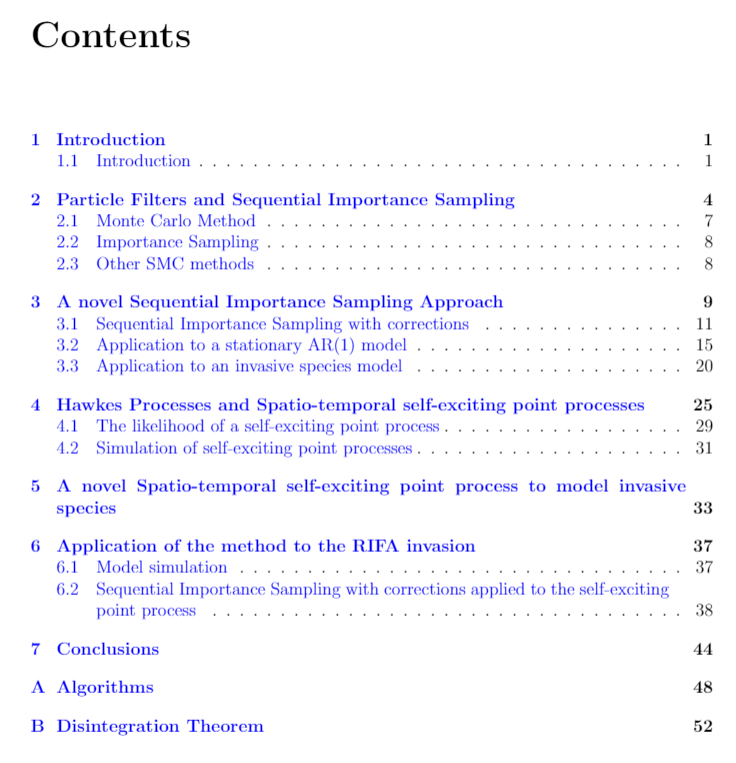
\includegraphics[scale=1]{Milestones/ContentsThesis.PNG}
\end{figure}

\section{Timeline}

I am planning to complete my master in the first half of 2021, in advance of the deadline (06/04/2022) and will apply for the PhD program pending the panel advice.

Outstanding work to complete the MPhil is:
\begin{itemize}
    \item Submit first paper (last week of January).
    \item Finalise code for second paper (February).
    \item Submit second paper (aiming for end of February).
    \item Finalise Introduction, conclusions and appendix of thesis. Check and fix existing chapters (March).
\end{itemize}

I am attaching to this document the first paper, the draft of the second paper and chapter 4 of the thesis.

The code for this project can be found at \url{https://github.com/valeaussie}.

\begin{figure*} [h!]
    \textbf{SIS with correction method compared with gold standard for an AR(1) model }\par\medskip
    \subfloat[fig 1]{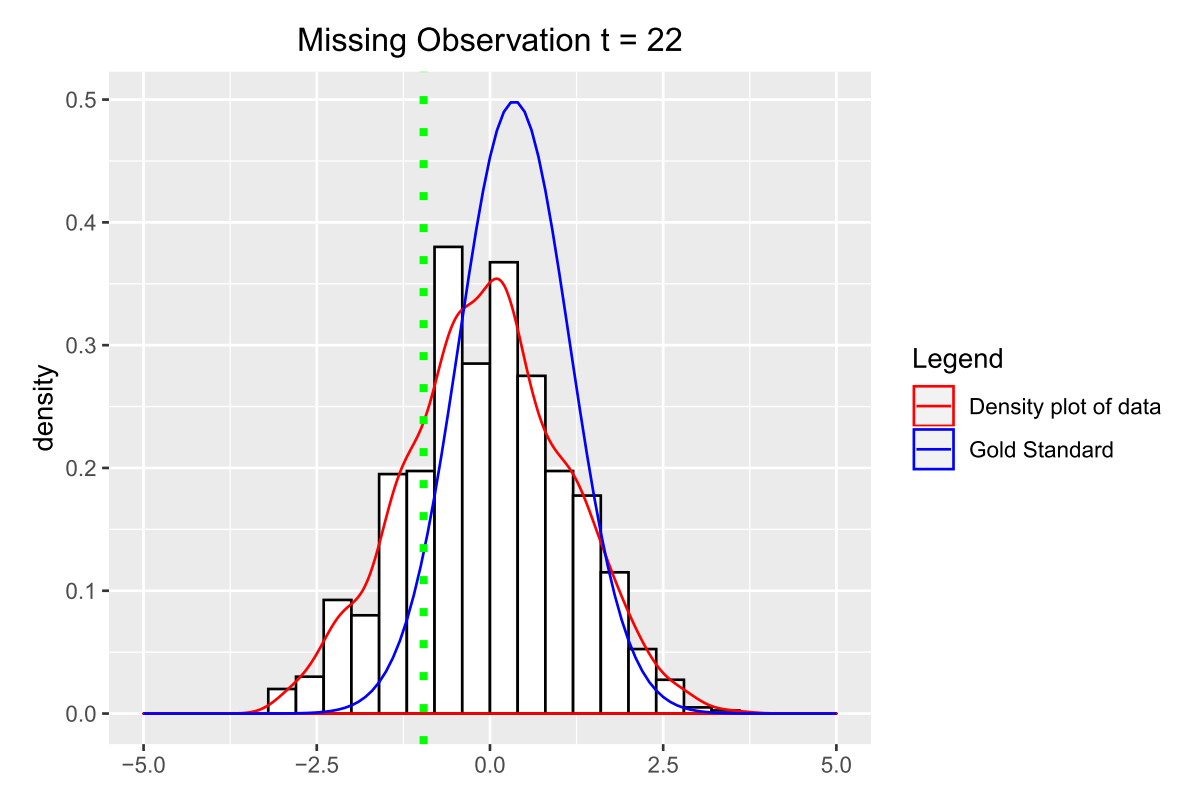
\includegraphics[width=0.5\linewidth]{Thesis/ar1_001.PNG}}
    \subfloat[fig 2]{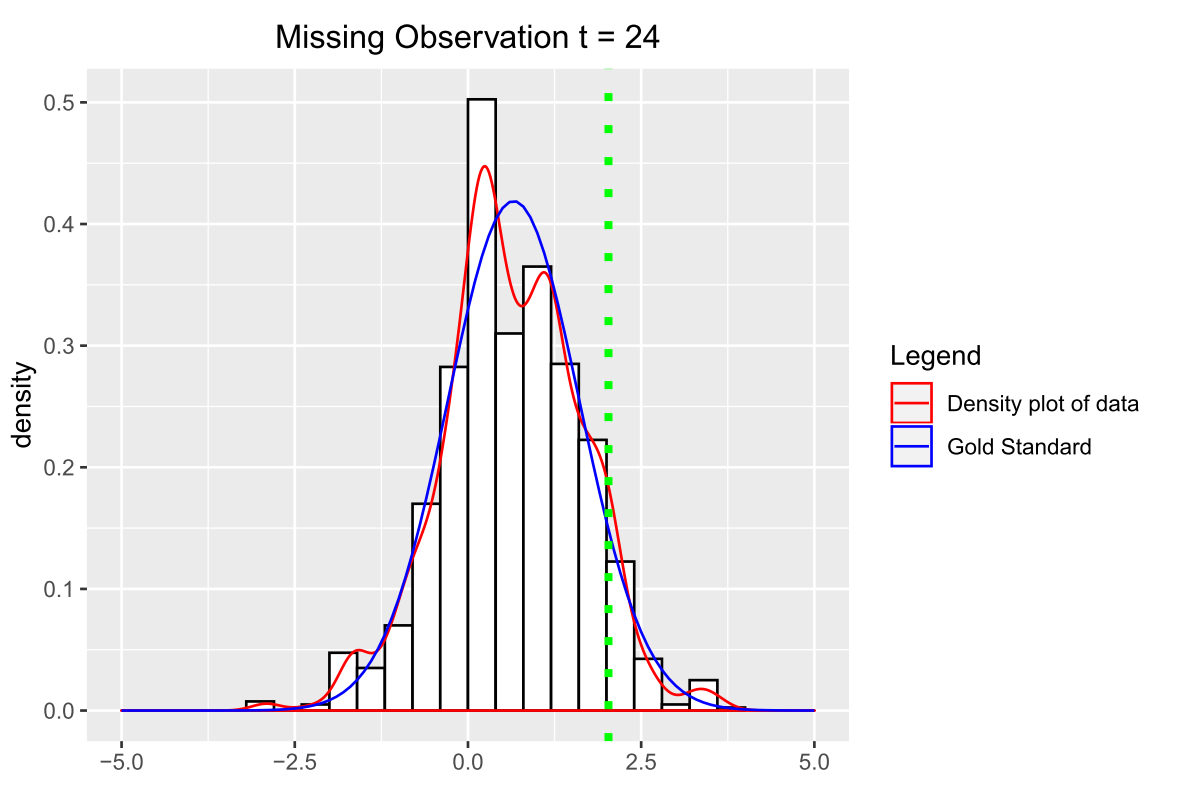
\includegraphics[width=0.5\linewidth]{Thesis/ar1_002.PNG}}\\
    \subfloat[fig 3]{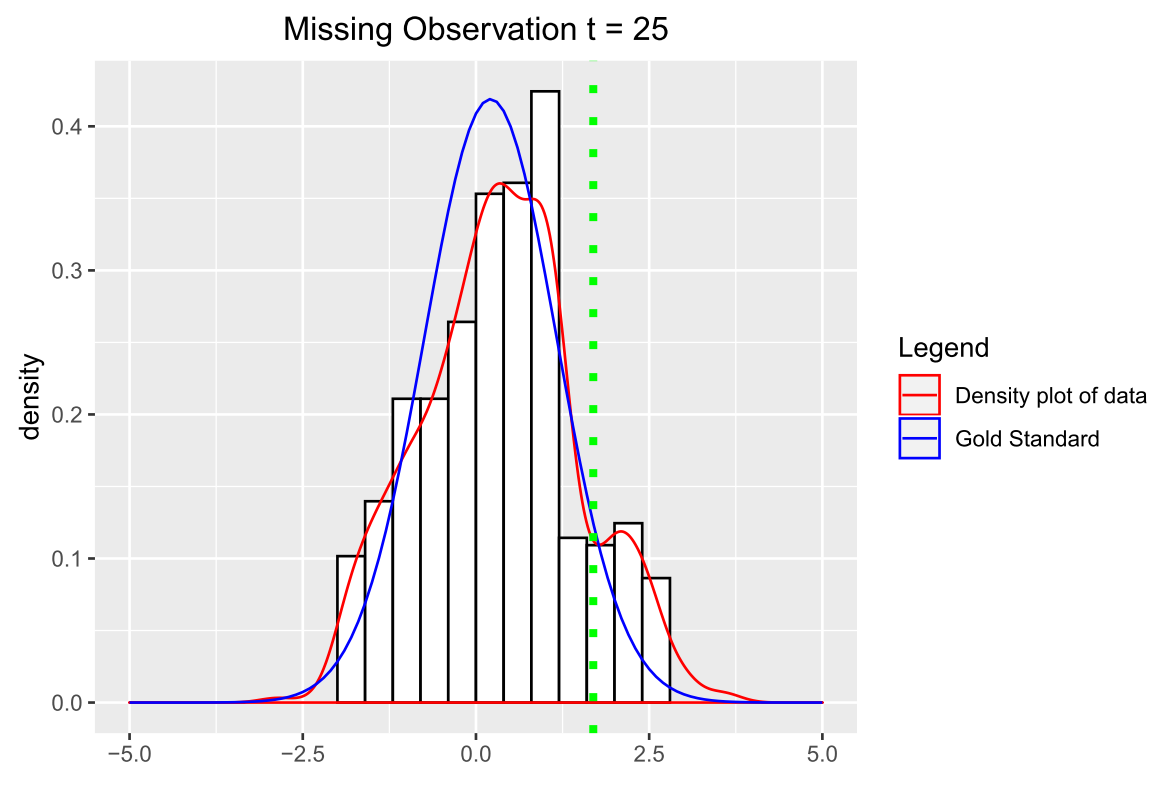
\includegraphics[width=0.5\linewidth]{Thesis/ar1_003.PNG}}
    \subfloat[fig 4]{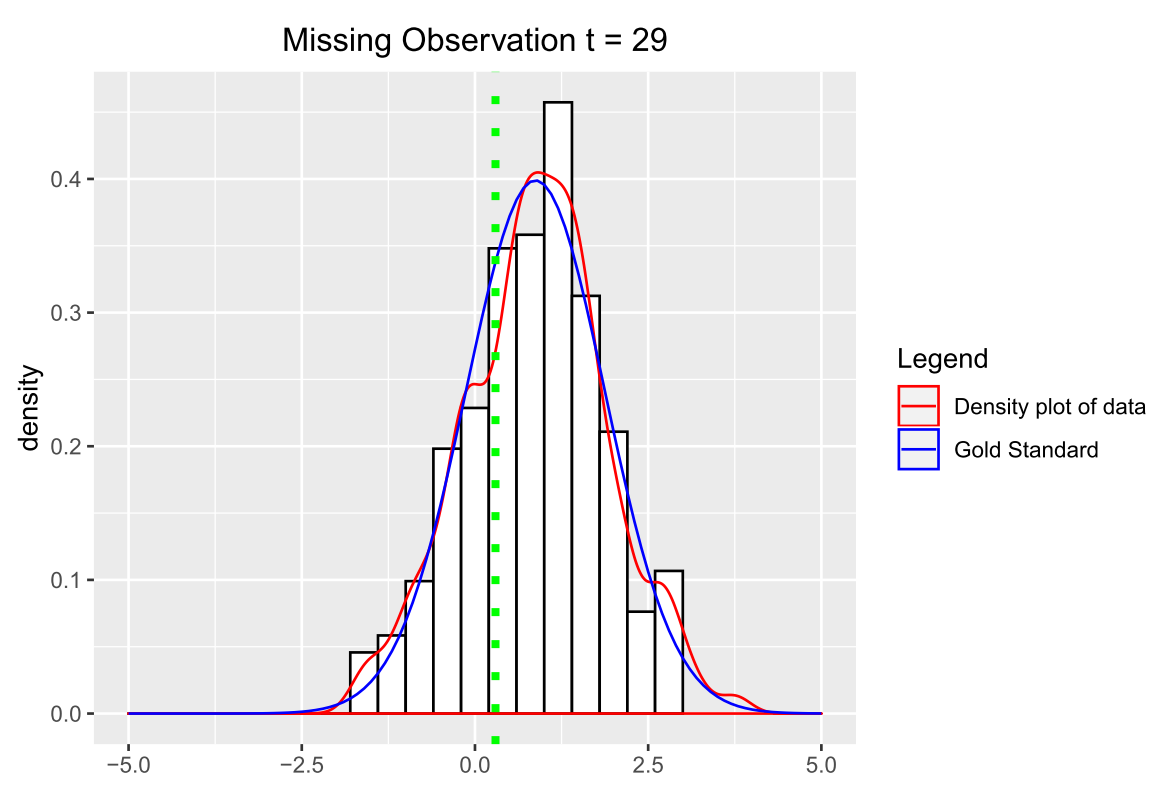
\includegraphics[width=0.5\linewidth]{Thesis/ar1_004.PNG}}\\
    \subfloat[fig 5]{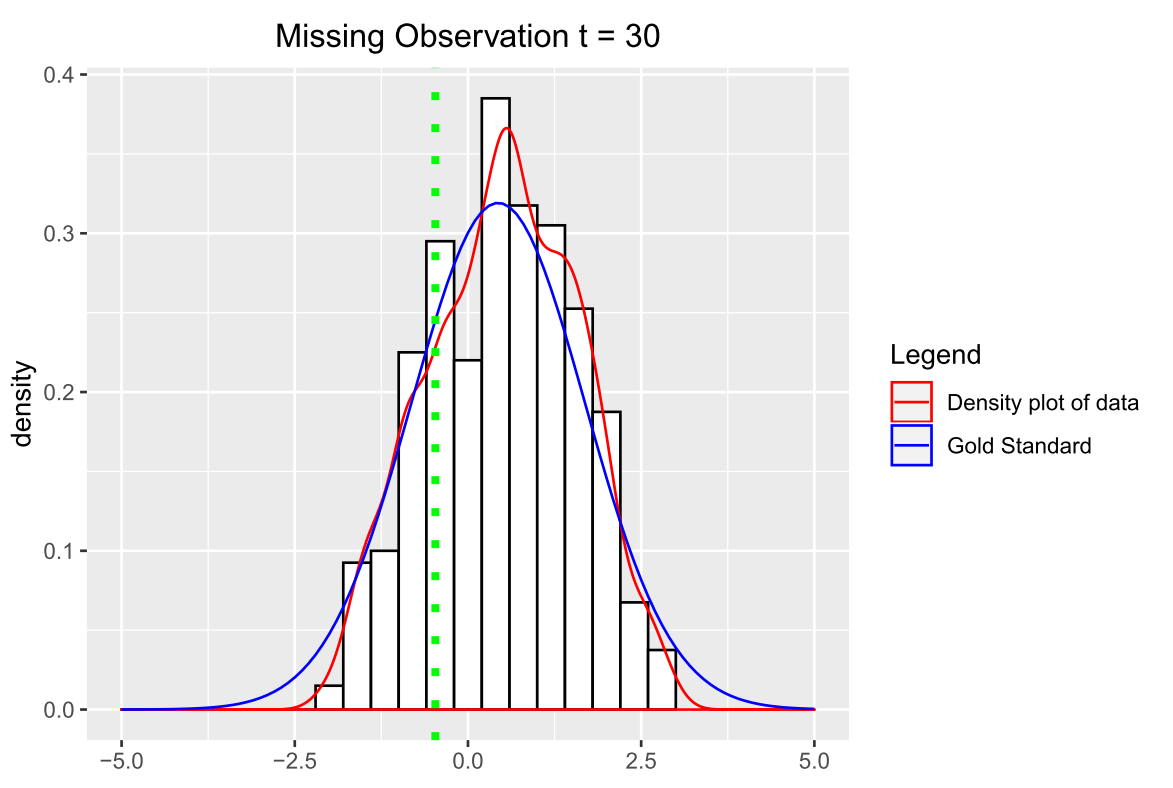
\includegraphics[width=0.5\linewidth]{Thesis/ar1_005.PNG}}
    \caption{AR(1) MODEL: Simulations with 1,000 particles and 30 times compared to the gold standard for the 5 missing times of the AR(1) model. In Green the value for the observation. The AR(1) model had parameter $\varphi = 0.5$, variance $\sigma^2 = 1$. The Bernoulli distribution had parameter $p = 0.2$}
\label{fig:1}
\end{figure*}

\begin{figure*} [h!]
    \textbf{SIS with correction simulation method applied to a simulated river invasion }\par\medskip
    \includegraphics[width=\textwidth]{Thesis/river_007.png}
    \caption{RIVER INVASION: Simulations with 1,000 particles and 50 cells of 3 possible river invasions all with probability of invasion $\theta = 0.3$ but with different values of the parameter $\varphi$ for the probability of the observations. Figures A1, B1 and C1 show the simulations of the 3 invasions while figures A2, B2 and C2 show the same simulations but with the observations superimposed in red. A1 and A2 show the invasion with $\varphi = 0.3$, B1 and B2 show the invasion with $\varphi = 0.1$. Figure C1 and C2 show the invasion with $\varphi = 0.8$.}
    \label{fig:2}
\end{figure*}


\end{document}
